% AB=AC=AD. The numerical coordinates are only a schematic layout, not source measurements.
% Both circles are tangent to AD at D; M1 is tangent to AB at B and M2 to AC at C.
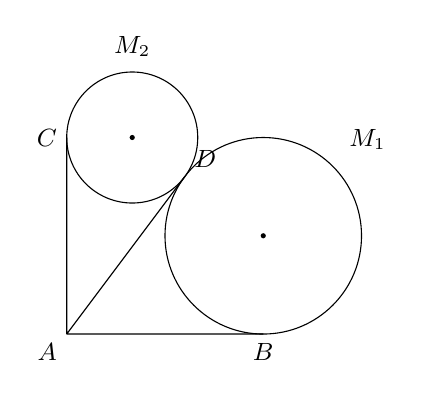
\begin{tikzpicture}[scale=0.78, every node/.style={font=\small}]
  \def\L{3.2}
  % 不标示意角度或长度数值，不把图示比例作为新增题设。
  \pgfmathsetmacro{\Dxx}{0.6*\L}
  \pgfmathsetmacro{\Dyy}{0.8*\L}
  \pgfmathsetmacro{\rOne}{0.5*\L}
  \pgfmathsetmacro{\rTwo}{\L/3}

  \coordinate (A) at (0,0);
  \coordinate (B) at (\L,0);
  \coordinate (C) at (0,\L);
  \coordinate (D) at (\Dxx,\Dyy);
  \coordinate (Mone) at (\L,\rOne);
  \coordinate (Mtwo) at (\rTwo,\L);
  \coordinate (MoneLabel) at ({\L+0.72*\rOne},{\rOne+0.72*\rOne});
  \coordinate (MtwoLabel) at (\rTwo,{\L+\rTwo});

  \draw (A) -- (B) (A) -- (C) (A) -- (D);
  \draw (Mone) circle (\rOne);
  \draw (Mtwo) circle (\rTwo);
  \fill (Mone) circle (1.2pt);
  \fill (Mtwo) circle (1.2pt);

  \node[below left] at (A) {$A$};
  \node[below] at (B) {$B$};
  \node[left] at (C) {$C$};
  \node[above right] at (D) {$D$};
  \node[above right=2pt] at (MoneLabel) {$M_1$};
  \node[above=2pt] at (MtwoLabel) {$M_2$};
\end{tikzpicture}
